\begin{enumerate}
  
	\item Provide in depth detailed review of previous work on abstractions. What can be applied to 3D printing and how?
	
		We will understand \emph{abstraction} as it is defined by \cite{Mi2009}. Abstraction is an strategic simplification and elimination of detail of a shape  keeping the visual appearance so that a viewer still understand the shape.
		
		For example, in \cite{Berger2013} they learn a particular artist style, and use it to create abstractions of portraits photographs which resembles a sketch of that particular artist.
		
		In \cite{DeGoes2011} they create abstraction of meshes by first segmenting the mesh on meaningful patches and then lower the level of detail of each patch, their main weakness is the need of the user for the initial segmentation. 
		
		In \cite{Li2010} the take an input mesh of a building and then they create an abstraction if the form of a \emph{Pop-Up} model of the building. 
		
		The work of \cite{Hildebrand2012} use also on meshes, and they create an abstraction of the meshe by planar cuts.
		it is a first step on abstraction using perceptual metric for fabrication, although their domain is very different from us. 
		
		Another example of abstraction based on meshes with the purpose of fabrication \cite{McCrae2011} where they create proxy’s from meshes with the propose of creating a puppet made of planar slices of the mesh.
		
		A first and very basic attempt to incorporate saliency into mesh abstraction was made on \cite{Yang2009} it is closely related to the problem. However, they only provide results form the saliency computation and not from the abstraction. 
		
		A precursor of our work is \cite{Mehra2009}, they start with an input mesh where they create a voxel hull and then they are able to make a network of curves. Their main weakness is that they claim to work only on man made objects.
		
		The work of \cite{Yumer2012}, is without a questions the closest to our. It builds on the previous~\cite{Mehra2009} however instead of creating the curve network they use an implicit surfaces approach to create the abstraction which is both simpler and useful on a more general range of objects. They have also a very interesting contribution: what they call they \emph{coabstraction}; they are able to module the grade of abstraction to be able to distinguish features between a specific given set of meshes.
	

  \item Provide review of previous work on perception in CG and how it can be applied to the problem of 3D printing.
	
	In the field of digital image processing, saliency is a number assigned to each pixel in the image that represents his visual importance. However, in the work of \cite{Kim2010} they bridge saliency metric with the perceptions of the visual quality of a mesh. They use a centric approach based on the geometry of the mesh to make the computation. They validate the results with an user study.
	
	Given a 3D scene the work of \cite{Feixas2009}, calculates the saliency of a mesh and then uses the information to find the best point of view of the scene. 
	
	In the work \cite{Wu2013} they create a method to calculate the saliency based on local feature and a global metric that they name rarity. They validate their results wit an user study.
	
	In the field of 3D printing \cite{Wang2015} they segment an object in pieces to optimize the printing time and at the same time use the saliency for printing the parts in an orientation to optimize the quality of the visible surface. They rely on adaptive slicing for performing this optimization which a feature that not in all the printer we can calculate.
	
	Opposed to our work is the work of \cite{Torkhani2015}, where they claim that if the mesh changes dynamically (for example in animation) the quality can be reduced. In this sense the p5roblem of 3D printing is the worst case, an static mesh, therefore the visual quality is very important.
	
	The work of \cite{Echevarria2014} is an example of a work focused on 3D printing using perception metric. However, they are focused on the narrow problem of printing hair of human figurines.
	
  \item Provide detailed pipeline of your method with a detailed time line of work. What, when, and how will be completed.
	
	\begin{figure}[htp]
		\centering
    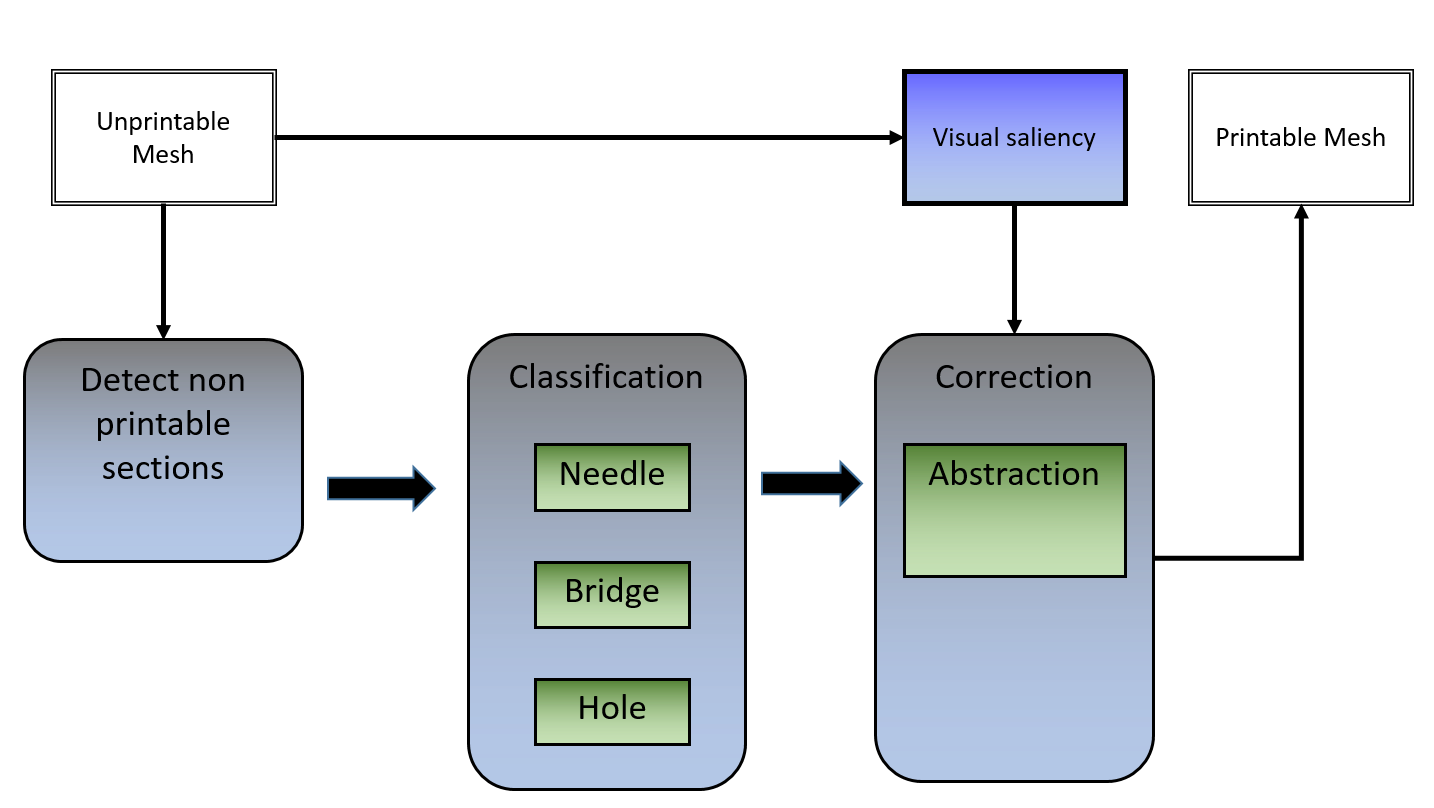
\includegraphics[width=0.85\textwidth]{img/Pipeline2}
		\caption{Proposed solution pipeline. White boxes are input and outputs. Blue boxes represents data and gray boxes represent process. The green boxes represents sub process}
		\label{fig:pipeline}
	\end{figure}
	
	The overview of the solution can be seen in Figure\ref{fig:pipeline}. The input is an unprintable mesh, which is use to calculate saliency and then is processed for the automatic detection of problematic parts. As is done in~\cite{Telea2011}, we covert the input mesh in a volumetric representation and then we use morphological operations to detect features small enough to print correctly which are mark as problematic.
	
	The problematic parts are classified using their topological properties into three categories: bridges, needles and holes. Then the part is corrected by abstraction according to the corresponding category and their corresponding saliency. Finally a new mesh is extracted from the volumetric representation as a final output.
	
	%Tim Mcgraw
	\item What specific volumetric representation do you propose to use?
	
	We create a simple voxelization of the original mesh by inscribing the model in a simple cubic grid. In other works we chose a $\Gamma \subset \mathbb{Z}^3$defined as follows: 
	
	\begin{equation}
		\Gamma = \left\lbrace \textbf{k} | A_i \leq k_i \leq B_i \text{ para } 1 \leq i \leq 3 \text{ whit } A_i < B_i \text{ and } A_i, B_i \in \mathbb{Z} 	\right\rbrace 
		\label{eq:scene}.
\end{equation}

	And then for each $\textbf{k} \in \Gamma$, we choose a positive real number $\Delta$ to define our voxels as:
	
	\begin{equation}
		\text{Vox} (\textbf{k}) = \left\lbrace \textbf{x} \in \mathbb{R}^3 | \Delta \left(  k_i - \dfrac{1}{2} \right) \leq x_i < \Delta \left(  k_i + \dfrac{1}{2} \right)  , \text{ for } 1 \leq i \leq 3 \right\rbrace 
		\label{ec:voxel}
	\end{equation}
	
	The number $\Delta$ is going to be our sampling distance. Four our need we will set $\Delta$ to half of the printer resolution, which in our case printers $\Delta = 0.25$mm. In order to perform the voxelization we use the method described in~\cite{Nooruddin2003}, which is implemented in Binbox\cite{Min2016}.
	
	\item What is the termination criterion? (How do you know when you are done?) Is it the user's choice, or automatic?
	
	There is no termination criteria in the sense of optimization. Rather we detect the problematic parts correct one by one and finish when there are no more problematic parts to correct. The user can choose to accept or reject the proposed abstraction, but regardless of his choose the abstraction is not recalculated.
	
	At one of the subprocess, when we produce the abstraction based on saliency there is an optimization of the metric of how far are from the original mesh. And in that sense there is a fix number of iterations of the abstraction as a termination criteria. Again it does not make sense become closer than $\Delta$

  \item Do you need to convert from volumetric representation back into to a mesh to print?
	%Theory not necesarry practice I do but is only an implementation detail. I use artzy algoritm to go back and forth between the two representations
	
	In theory, this will be not necessary since most 3D printers need to slice a model and then raster each slice. However, since we want to keep the process independent from the printer, we are not able to send the slicing directly. Instead, we convert back to a mesh representation as can be seen in Figure~\ref{fig:pipeline} the output is a mesh.
	
	In order to extract a mesh from the volumetric representation we use the surface tracking algorithm described in~\cite{Artzy1980}, which guaranties topology correction, and fairly regular meshes.
  
	\item Can you elaborate more about this perception metric you will use to evaluate visual saliency of the 3D printed object? Are you going to verify your metric with user study? e.g. to see if user will also say that corrected model is visually plausible after the modification and there is no obvious better way how to perform the correction?
	
	This is a very interesting question. I'm not sure, the work of already evaluated the quality of saliency as a perception metric in 3D meshs, in 3D printed figurines the same result should apply. 
	
	Also, remember that the modification of the mesh is local to the problematic part. So, besides to show the difference in saliency in the original mesh and the corrected mesh; I don't know what else to measure.
	
	Given said that, the user study for the final result is not completely of the table.
	
	\item How will you combine perceptual optimization with structural/material optimization? I understand we want to have optimized object that is visually plausible, but we still have to keep printability and structural strength.
	
	I’m only clamming possible contribution in the terms of printability. And I'm just measuring the printability in the terms of printer resolution. I'm aware that the result might need to be combined with a post processing step to ensure structural strength. Maybe even use the stress relive~\cite{Stava2012} as a post processing step.
	
	The structural strength extension is an interesting problem by itself if you don't want to modify the mesh that much and abstraction sounds like a very powerful tool to attack the problem. However right now is out of the scope of this work.
	
	\item You mentioned that you would like to have the process interactive. I assume GPU acceleration will be used in this case. Since the model will be volumetric, how would you cope with memory restrictions put on fully volumetric (voxel) model?
	%Yes, this is a great question too. Voxelization is made in CPU, but then the represetation used is morphological, so it is not really that memory consumed. So far in they say thta the expense step is, which right now is made in CPU and is still good. So I guess it is not a concer right now. I do have some cad ounder the sleeve if this is a bootle neck later.
	This is a great question too. We have two advantages. 
	
	First that as we can see in~\cite{Telea2011} the most expensive part should be the thin region detections, we can do in less than 10s, in a CPU implementation for a $1024^3$ discretization that given the printer resolution is enough for a 20cm print.
	
	Second, the correction is per problematic part (a connected component), and this are handles in the morphological representation. So the memory requirements should not be as high as it will be if we load the original volume in GPU.
		
\end{enumerate}